\documentclass[10pt,twocolumn,letterpaper]{article}
\def\code#1{\texttt{#1}}
\usepackage{natbib}
%% Language and font encodings
\usepackage[french]{babel}
\usepackage[utf8x]{inputenc}
\usepackage[T1]{fontenc}
\usepackage{float}
%% Sets page size and margins
\usepackage[a4paper,top=3cm,bottom=2cm,left=3cm,right=3cm,marginparwidth=1.75cm]{geometry}
%% More packages
\usepackage{amsmath}
\usepackage{graphicx}
\usepackage[colorinlistoftodos]{todonotes}
\usepackage[colorlinks=true, allcolors=blue]{hyperref}
\usepackage{fancyhdr}
\pagestyle{fancy}
\fancyhead[R]{Ms HPC-AI}

\bibliographystyle{unsrt}
%% Title
\title{
		\usefont{OT1}{bch}{b}{n}
		\normalfont \normalsize \textsc{Mines ParisTech - Ms HPC-AI} \\ [10pt]
		\huge Projet d'Algèbre Linéaire Distribuée :\\ Profiling de BoomerAMG \\
}
\selectlanguage{french}
\usepackage{authblk}
\author{Julian AURIAC \& Aymeric MILLAN}
\affil{Cours de Christophe BOVET}
\date{17 Janvier 2022}
\begin{document}

%% just to make warning go away. Adjust the value after looking into the warning
\setlength\headheight{26pt}
% \rhead{{\color{blue}\rule{1cm}{1cm}}}

\lhead{
\includegraphics[width=4cm]{fig/Logo_Mines_ParisTech.svg.png}}

\maketitle

%%%%%%%%%%%%%%%%%%%%%%%%%%%%%%%%%%%%%%%%%%%%%%%%%%%%%%%%%%%%%%%%%%%%%%%%%%%%%%%%
%%%%%%%%%%%%%%%%%%%%%%%%%%%%%%%%%%%%%%%%%%%%%%%%%%%%%%%%%%%%%%%%%%%%%%%%%%%%%%%%
%% RESUME
\begin{abstract}
Voici le document regroupant nos benchmarks de
\href{https://hypre.readthedocs.io/en/latest/solvers-boomeramg.html}{BoomerAMG},
inclus dans la librairie
\href{https://hypre.readthedocs.io/en/latest/index.html}{HYPRE}.

L'objectif du projet est double : il s'agit d'abord d'appliquer les méthodes de
résolutions multigrilles algébriques de BoomerAMG sur des
\href{https://sparse.tamu.edu/}{matrices de problématiques réelles} au format
\code{.mtx} (Matrix Market).
Le deuxième objectif du projet est la réalisation d'études
d'extensibilités :
\begin{description}
    \item [Forte :] Avec
\href{https://sparse.tamu.edu/Janna/Emilia_923}{un problème de taille fiche}
au format Matrix Market, nous augmentons le nombre de processus MPI.
    \item [Faible :] En partant de $1$ processus MPI et
d'un problème de taille $n \times n$, nous doublons la taille du problème
\textbf{et} le nombre de CPU qui travaillent sur le problème.
\end{description}

Nous mesurons dans les deux cas les temps d'exécutions de la résolution d'un
système de la forme $Au = f$, avec $A$ la matrice de départ (i.e l'observation),
$f$ la solution vers laquelle on veut converger (i.e le résultat) et $u$
le système que l'on cherche à trouver.

En plus de ces outils, ce projet apporte une vision générale sur les
méthodologies de développement sur des clusters de calculs comme celui du CEMEF.
Nous avons pu approfondir les concepts tels que la réservation des coeurs de
calcul, le partage de ressources ou encore les scripts automatisés,
ici avec le scheduler \code{OAR}.
\end{abstract}

%%%%%%%%%%%%%%%%%%%%%%%%%%%%%%%%%%%%%%%%%%%%%%%%%%%%%%%%%%%%%%%%%%%%%%%%%%%%%%%%
%%%%%%%%%%%%%%%%%%%%%%%%%%%%%%%%%%%%%%%%%%%%%%%%%%%%%%%%%%%%%%%%%%%%%%%%%%%%%%%%
%% RECUPERER LE CODE
\section{Récupérer le code}
Le code est disponible sur
\href{https://github.com/Aympab/HypreBoomerAMG_Benchmark}{ce repo GitHub}.
Vous pourrez aussi trouver le code et une archive dans nos repertoires
personnels sur le CEMEF. Le programme est déjà compilé sur le cluster.

Nous avons ajouté l'option \code{-file} à l'exécution qui permet de préciser
un chemin d'accès relatif vers un fichier au format .mtx. Le code fonctionne
pour des \textbf{matrices carrées} uniquement. De plus, avec les options par
défaut (e.g \code{-gamma}, le cycle AMG utilisé, V par défaut), seulement les
matrices symétriques définies positives permettent de converger vers une
solution. Nous avons téléchargé quelques matrices de ce type dans le répertoire
\code{matrices}, à la racine du projet.

%%%%%%%%%%%%%%%%%%%%%%%%%%%%%%%%%%%%%%%%%%%%%%%%%%%%%%%%%%%%%%%%%%%%%%%%%%%%%%%%
%%%%%%%%%%%%%%%%%%%%%%%%%%%%%%%%%%%%%%%%%%%%%%%%%%%%%%%%%%%%%%%%%%%%%%%%%%%%%%%%
%% Implémentation
\section{Logique d'implémentation}

Pour le benchmarking, nous avons utilisé un script shell qui formate les données
des logs OAR en fichiers csv.
Ensuite, à l'aide de python et surtout de la librairie \code{pandas}, nous avons
traité les données pour les visualiser ici.
Les données brutes sont disponibles dans le répertoire \code{log/} du projet.

Pour ce qui est de la lecture de fichier \code{.mtx} et le découpage sur les
différents coeurs de calculs, nous avons utilisé la librairie
\href{https://eigen.tuxfamily.org/index.php?title=Main_Page}{Eigen}.
La difficulté était premièrement de s'approprier la librairie, notamment les
méthodes pour accéder aux données brutes (i.e. \code{raw buffers}), dans le but
de les envoyer à l'autre librairie, HYPRE. L'interfaçage entre les deux
librairies ainsi que le découpage de la matrice pour les différents processus
MPI ont été pour nous des difficultés notables de ce projet (et donc des axes
d'amélioration).

Nous avons essayé de réutiliser au maximum le code qui était déjà développé par
le professeur, vous trouverez le code commenté dans le fichier \code{tp.cpp}.


%%%%%%%%%%%%%%%%%%%%%%%%%%%%%%%%%%%%%%%%%%%%%%%%%%%%%%%%%%%%%%%%%%%%%%%%%%%%%%%%
%%%%%%%%%%%%%%%%%%%%%%%%%%%%%%%%%%%%%%%%%%%%%%%%%%%%%%%%%%%%%%%%%%%%%%%%%%%%%%%%
%% ETUDE STRONG
\section{Étude d'extensibilité forte}

Dans cette partie, nous avons utilisé la matrice
\href{https://sparse.tamu.edu/Janna/Emilia_923}{Emilia923}, qui est issue d'un
problème de géomécanique. C'est une matrice symétrique définie positive avec
environ $4\times 10^6$ nnz., et $923136$ lignes et colonnes.

\begin{figure}[H]
  \centering
  \caption{Profil de Emilia923}
  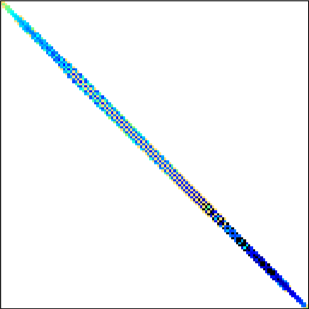
\includegraphics[width=0.3\textwidth]{fig/Emilia923.png}
\end{figure}

En gardant ce même problème tout au long de l'étude, nous allons augmenter
le nombre de processus MPI en parralèle. Nous montons jusqu'à $3 \times 28 = 84$
processus car cela correspond à $3$ noeuds de calcul du cluster CEMEF complets.
Nous avons délimité par la ligne horizontale rouge le nombre de coeurs pour un
même noeud.
Voici les résultats de ces exécutions :

\begin{figure}[H]
    \centering
    \caption{Étude d'extensibilité forte}
    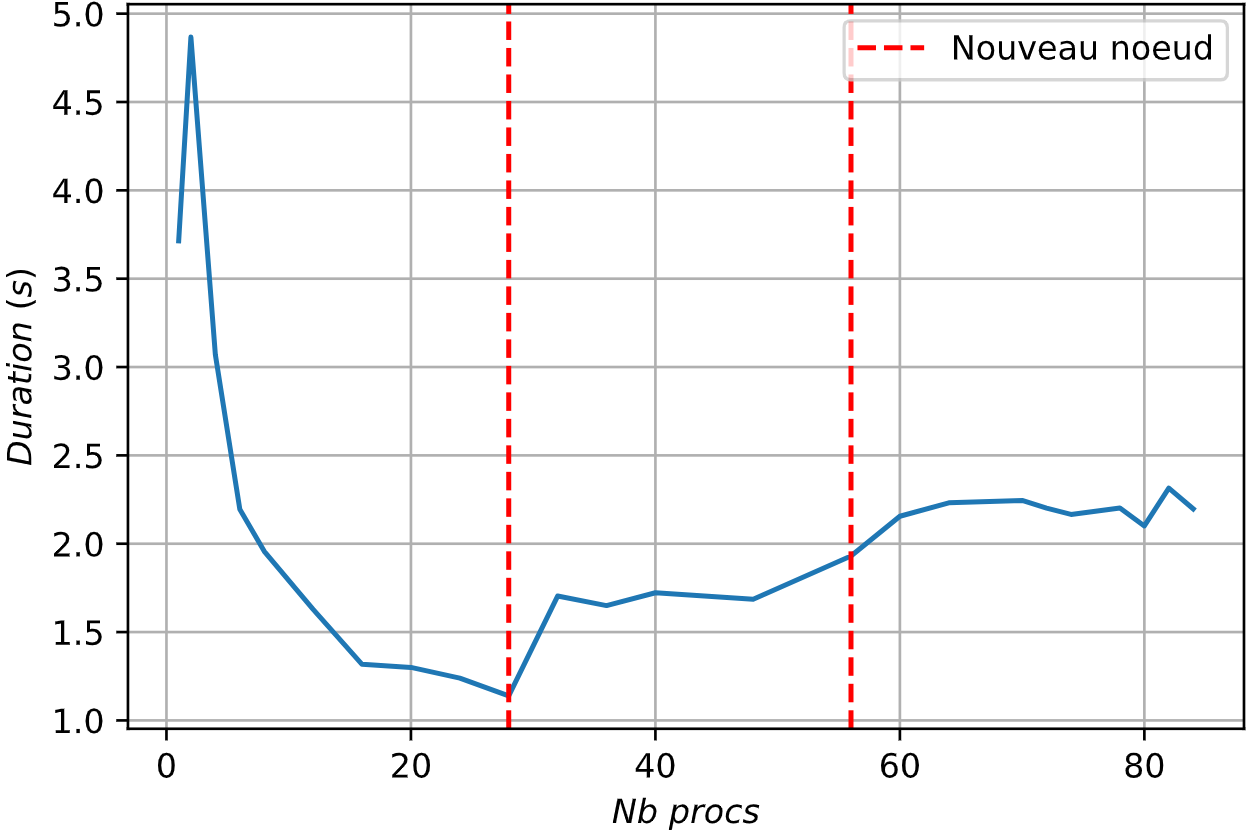
\includegraphics[width=0.45\textwidth]{fig/strong_scalab.png}
  \end{figure}

Une première chose assez flagrante que l'on peut remarquer ici est que dès que
l'on sort du même noeud de calcul, et que les communications MPI se font entre
différents noeuds, le temps de calcul augmente.
De plus, on peut voir une perte de performance notable lorsqu'on passe de 1 à 2
processus MPI. Cette étude a été réalisée avec les paramètres par défaut du
solveur.
Notons que nous avons pris soin de
réserver trois noeuds qui se trouvent côte a côte sur le cluster.

%%%%%%%%%%%%%%%%%%%%%%%%%%%%%%%%%%%%%%%%%%%%%%%%%%%%%%%%%%%%%%%%%%%%%%%%%%%%%%%%
%%%%%%%%%%%%%%%%%%%%%%%%%%%%%%%%%%%%%%%%%%%%%%%%%%%%%%%%%%%%%%%%%%%%%%%%%%%%%%%%
%% ETUDE
\section{Étude d'extensibilité faible}

Voici ci-après une étude d'extensibilité faible du programme. Une fois de plus,
les paramètres utilisés ici sont ceux par defauts : Cycle V, coarsening CLJP,
interpolation classique, un seul balayage par niveau, pas de coarsening aggresif
. Vous trouverez toutes les informations sur les paramètres par défaut dans le
code, et plus en détail sur le manuel de référence HYPRE.

\begin{figure}[H]
    \centering
    \caption{Étude d'extensibilité faible}
    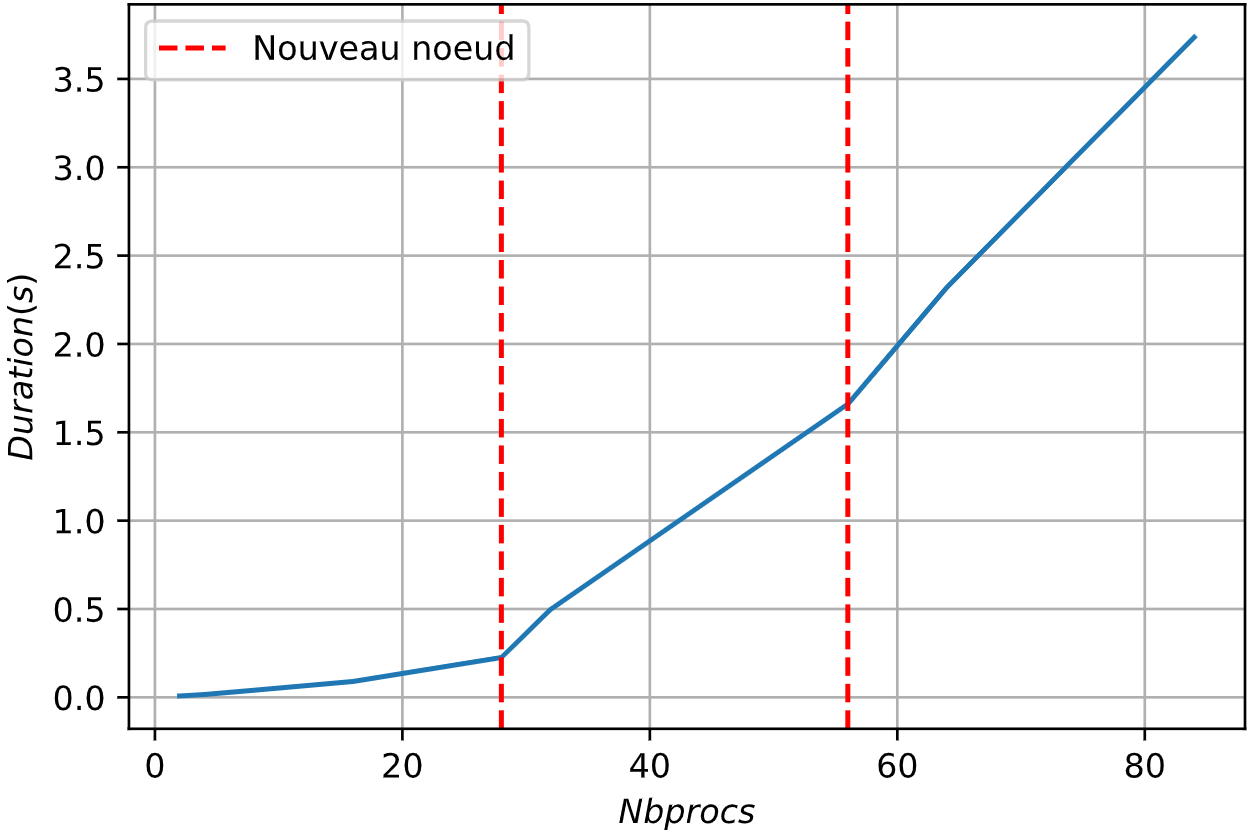
\includegraphics[width=0.45\textwidth]{fig/weak_scalab.png}
  \end{figure}

Une fois de plus, nous pouvons constater qu'il y a une divergence lorsque l'on
sort d'un seul et même noeud de calcul. Nous étudierons brièvement plus tard
ce phénomène. 
D'abord, nous allons jouer sur les paramètres de résolution du problème.


%%%%%%%%%%%%%%%%%%%%%%%%%%%%%%%%%%%%%%%%%%%%%%%%%%%%%%%%%%%%%%%%%%%%%%%%%%%%%%%%
%%%%%%%%%%%%%%%%%%%%%%%%%%%%%%%%%%%%%%%%%%%%%%%%%%%%%%%%%%%%%%%%%%%%%%%%%%%%%%%%
%% ETUDE PARAMETRES
\section{Changement des paramètres de base}

De nombreux paramètres sont disponibles dans la librairie BoomerAMG. Entre
autres, nous pouvons choisir la méthode de coarsening et d'interpolation.
Nous avons essayé d'utiliser des méthodes qui admettent possiblement une plus
grande marge d'erreur, mais qui sont tournées vers la performance.
Voici quelques temps d'exécutions en fonction de différents paramètres. Les
benchmarks de cette parties ont été réalisés sur $28$ coeurs en parallèle, tous
sur un seul et même noeud. La taille du problème est fixé à $8096^2$.

\begin{figure}[H]
  \centering
  \caption{Variation du Coarsen type}
  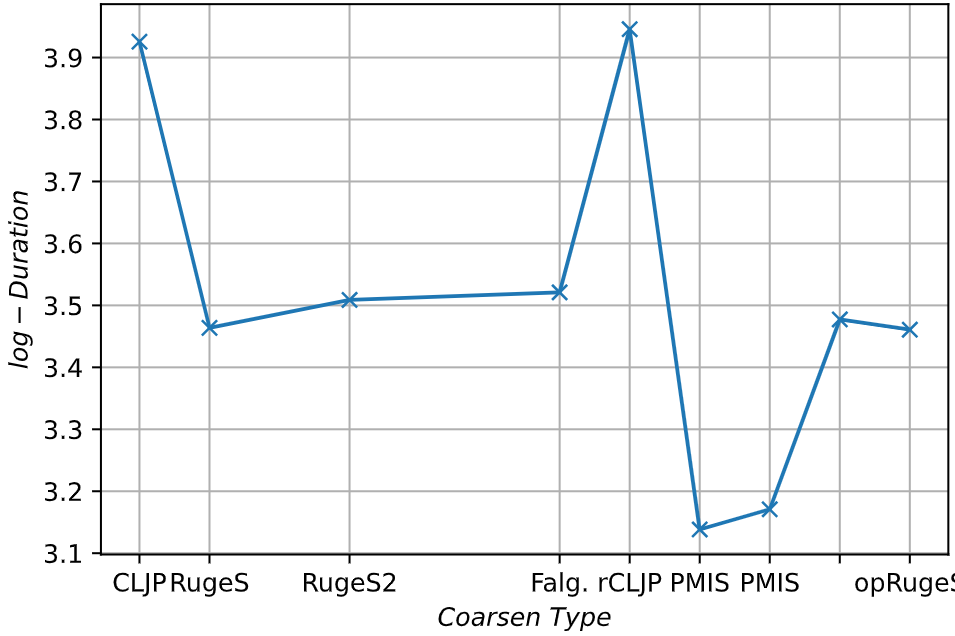
\includegraphics[width=0.45\textwidth]{fig/strong_coarsen_type.png}
\end{figure}

\begin{figure}[H]
    \centering
    \caption{Variation du aggressive coarsing}
    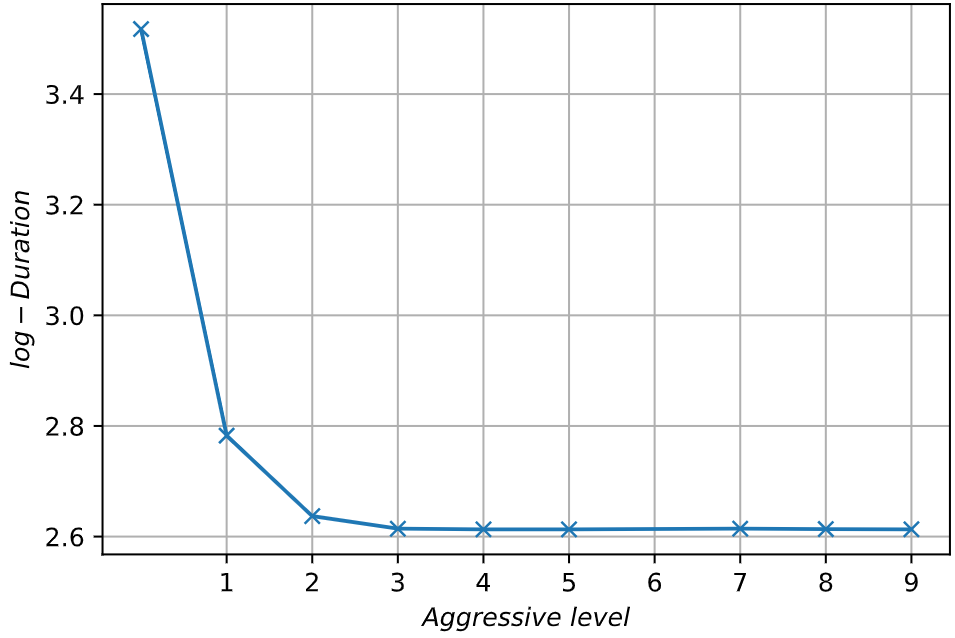
\includegraphics[width=0.45\textwidth]{fig/strong_agg_level.png}
  \end{figure}

  \begin{figure}[H]
    \centering
    \caption{Variation du smoother}
    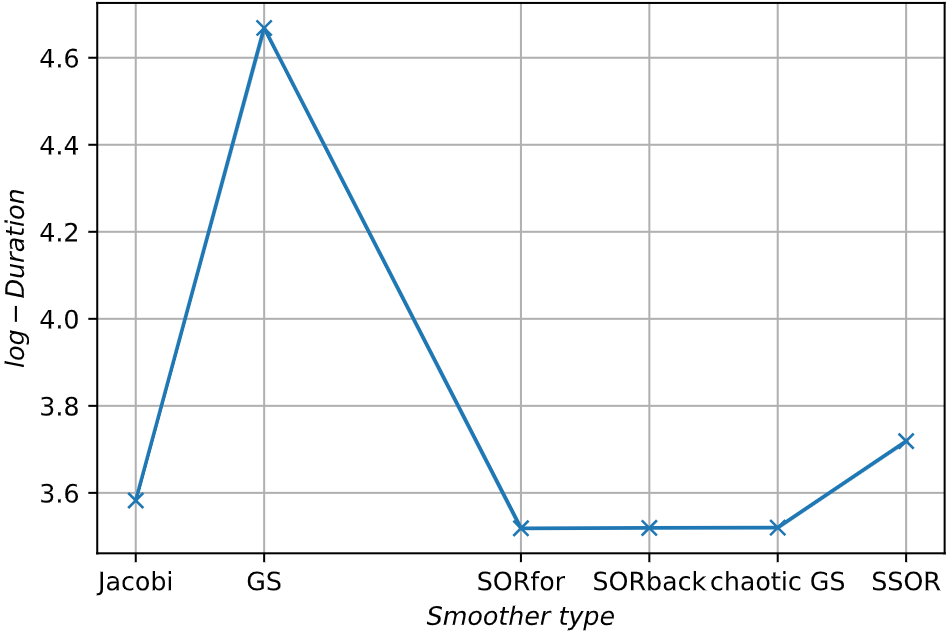
\includegraphics[width=0.45\textwidth]{fig/strong_smoother.png}
  \end{figure}

Il existe de nombreux autres paramètres qu'il faudrait étudier selon le profil
de la matrice que nous essayons de résoudre. Mais avec ce que nous avons testé,
et notre profil de matrice (symmétrique définie positive), nous allons combiner
les paramètres qui semblent minimiser le temps de calcul en se basant sur les
trois précédents graphiques, nous allons donc utiliser :

\begin{description}
  \item[Coarsening type] - Méthode utilisée pour réaliser le maillage grossier :
\href{https://hypre.readthedocs.io/en/latest/ch-references.html#dfny2008}{PMIS}
  \item[Aggresive coarsing] - Utilisé pour faire un maillage grossier de manière
aggressive, ce qui peut réduire les allocations mémoire et la complexité. Ici, 
nous allons réaliser un \textit{coarsing} aggressif sur 3 niveaux. 
  \item[Relaxation type] - Le lisseur à utiliser pour la phase de prélissage :
hybride Gauss-Seidel ou SOR, avec une résolution ascendante (\textit{forward
solve}).
\end{description}


Voici une comparaison entre le temps d'exécution du solveur avec les  paramètres
par défaut de HYPRE et les paramètres que nous avons choisis. Il s'agit d'une
étude d'extensibilité forte, nous gardons la même taille de problème que pour
les graphiques précédents.

\begin{figure}[H]
  \centering
  \caption{Comparaison des paramètres}
  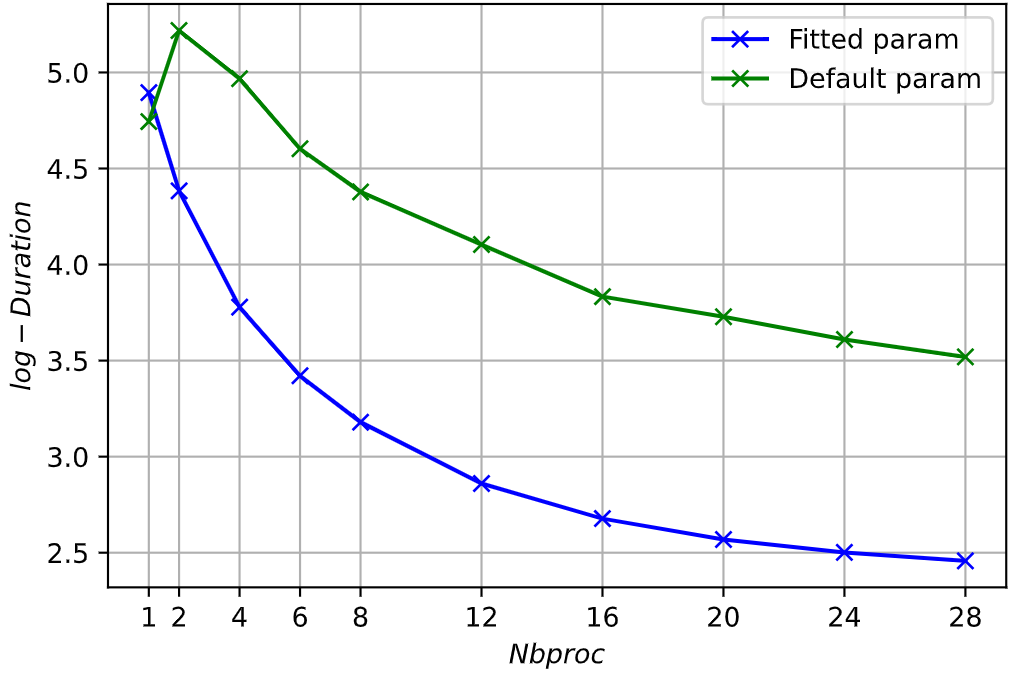
\includegraphics[width=0.45\textwidth]{fig/strong_best_param.png}
\end{figure}

La combinaison de ces trois paramètres semble donc être efficace sur ce type de
problème. Essayons maintenant de l'utiliser pour la résolution du problème
Emilia923, sur un plus grand nombre de coeurs : 

\begin{figure}[H]
  \centering
  \caption{Comparaison des paramètres sur Emilia923}
  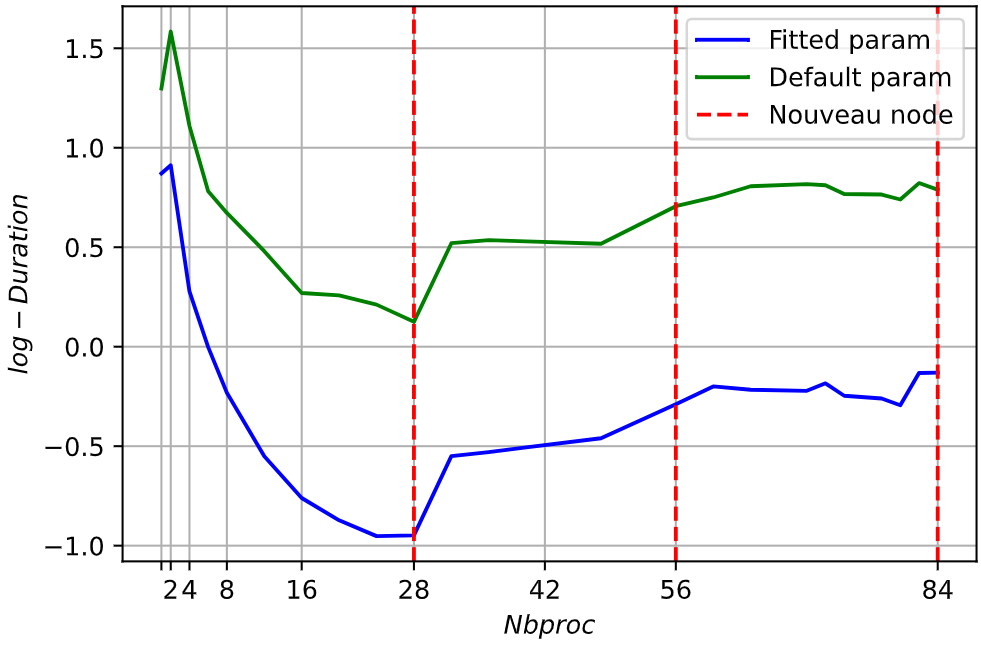
\includegraphics[width=0.45\textwidth]{fig/strong_best_param_emilia.png}
\end{figure}

Les résidus en fin de résolution sont du même ordre de grandeur tout le temps
($10^-9$), cependant, on peut constater avec le graphique suivant que le nombre
d'itérations par résolution augmente avec les paramètres fixés. Cela pourrait
être une piste pour essayer d'utiliser au mieux la librairie.

\begin{figure}[H]
  \centering
  \caption{Nombre d'itérations sur Emilia923}
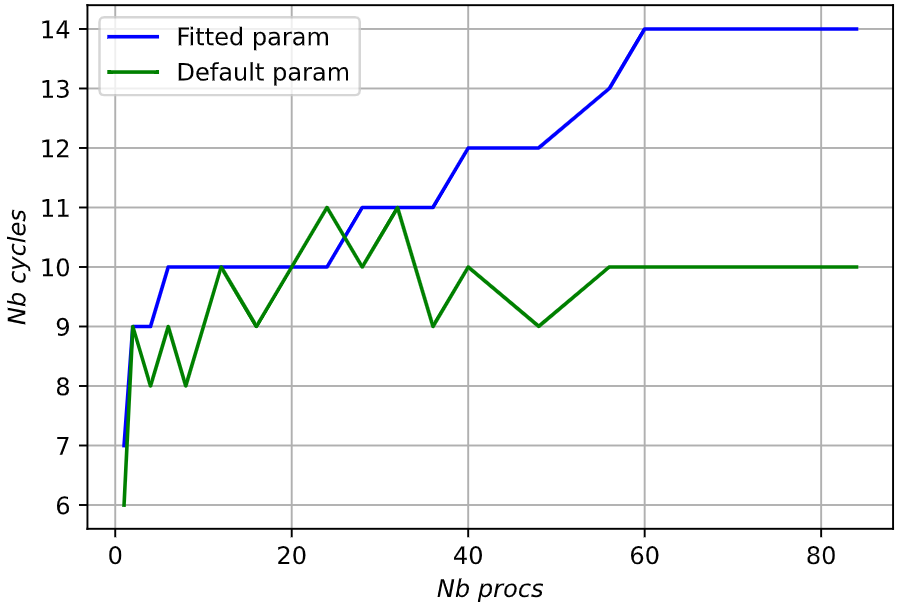
\includegraphics[width=0.45\textwidth]{fig/strong_best_param_emilia_nbiter.png}
\end{figure}

Nous pouvons constater que ces paramètres fonctionnent donc aussi bien sur ce
problème réel .mtx.
De plus, le pic que nous avions obtenus en passant de 1 processus
à 2 tend à s'effacer, probablement dû au fait de l'
\textit{aggressive coarsening}. Malgré tout, les communications inter-nodes
semblent impacter grandement les performances.

%%%%%%%%%%%%%%%%%%%%%%%%%%%%%%%%%%%%%%%%%%%%%%%%%%%%%%%%%%%%%%%%%%%%%%%%%%%%%%%%
%%%%%%%%%%%%%%%%%%%%%%%%%%%%%%%%%%%%%%%%%%%%%%%%%%%%%%%%%%%%%%%%%%%%%%%%%%%%%%%%
%% ETUDE DISTANCE
\section{Étude de l'impact de la distance entre deux noeuds sur le cluster
CEMEF}

Nous avons mis un certain temps avant de réaliser que certains de nos calculs
devenaient longs à cause de la séparation des CPUs sur plusieurs nodes. En effet
, en augmentant d'un le nombre de processus MPI, les calculs devenaient parfois
100x plus lents.

Nous avons d'abord pensé que la distance physique qui sépare les nodes dans
les quels se trouvent les différents CPU utilisés par MPI impactait les
performances. Pour en avoir le coeur net, nous avons décidé de réaliser l'étude.
suivante :
Il s'agit du temps de calcul pour un problème de taille fixe et pour \textbf{2}
processus MPI. L'idée est d'avoir deux CPUs qui sont bien sur deux noeuds
différents, et de faire varier la distance entre ces noeuds
(i.e. de choisir des noeuds plus éloignés physiquement sur le cluster à chaque
itération). Voici les résultats que nous avons obtenus :

\begin{figure}[H]
    \centering
    \caption{Impact de la distance entre les noeuds sur la performance}
    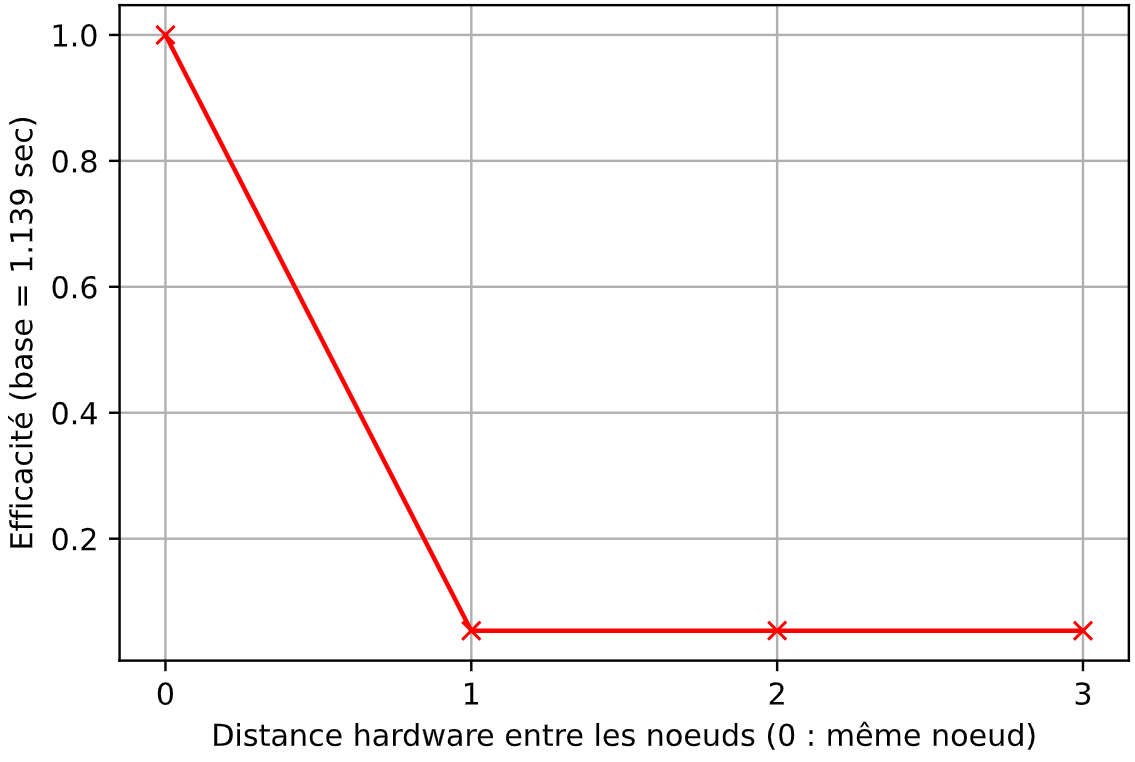
\includegraphics[width=0.50\textwidth]{fig/dist_profiling.png}
  \end{figure}

Comme nous pouvons le constater, notre hypothèse était fausse. La distance
physique qui sépare deux nodes n'impacte pas de manière significative les
performances. Cependant, nous pouvons voir que les performances sont
grandement affectées par le fait de sortir du même noeud de calcul.
Notre hypothèse est la suivante : comme les processus travaillent sur une
même mémoire RAM physique (au niveau hardware), malgré le fait que nous
utilisons de la programmation en mémoire distribuée, les communications MPI
sont largement optimisées. Entre autres, nous n'avons pas besoin d'accéder
au réseau. En conclusion, si notre problème peut rentrer dans la mémoire RAM
d'un seul noeud, il vaut mieux favoriser l'utilisation de tous les coeurs de
ce noeud plutôt que d'ajouter des coeurs de calculs qui seraient sur des noeuds
différents. Bien sûr, pour être sûr de cela, il faudrait faire une étude plus
approfondie, notamment en mesurant le temps des communications par rapport au
temps de calcul.

\section*{Conclusions}

Les courbes que nous obtenons avec les profilings d'extensibilité forte et
faible correspondent à ce que nous avions vu en cours.
L'étude "approfondie"
que nous avons mené nous a permis de découvrir de nouveaux aspects de la
programmation haute performance. Entre autres, nous avons pu clairement
ressentir l'impact des communications réseaux sur les performances.
Une fois les outils et les concepts (un peu) appropriés, nous nous sommes aussi
rendus compte du confort qu'apporte l'utilisation
d'une librairie telle que HYPRE,
qui masque l'implémentation des communications MPI. C'est quand même un niveau
d'abstraction qui rend la programmation assez agréable et rassurante, tout en
nous permettant de garder un contrôle sur la performance
car nous restons dans un langage bas niveau avec le C/C++.

\section*{Pistes d'amélioration}

\begin{itemize}
  \item Réaliser un découpage des matrices CSR par valeurs et non
par lignes, afin d'être sûr d'avoir une charge de calcul équilibrée entre les
processeurs. De plus, rendre le code plus générique en permettant de résoudre
des sytèmes qui ne sont pas des matrices carrées.
  \item Donner la possibilité d'importer le vecteur solution en
entrée du programme, comme pour la matrice de départ.
  \item Étude plus approfondie sur le coût des communications MPI.
  \item HYPRE donne la possibilité d'être utilisé sur GPU. Il aurait été intéressant de
comparer les performances entre une version CPU et une version GPU. Malgré nos
efforts, les versions de CUDA qui font tourner HYPRE sont anciennes
et ne tournent que sur des "vieux" systèmes d'exploitations (e.g. Ubuntu 16.04).
Ces versions ne sont pas disponibles sur les machines que nous avons à
disposition à l'école.
\end{itemize}

\bibliography{bibliography}
\end{document}
